\begin{frame}
  \frametitle{From Electrical Meter to Smart Meter}
%  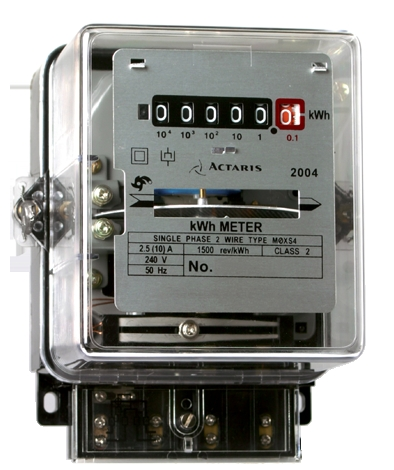
\includegraphics[width=.5\textwidth]{graphics/electrical_meter.jpg}

%  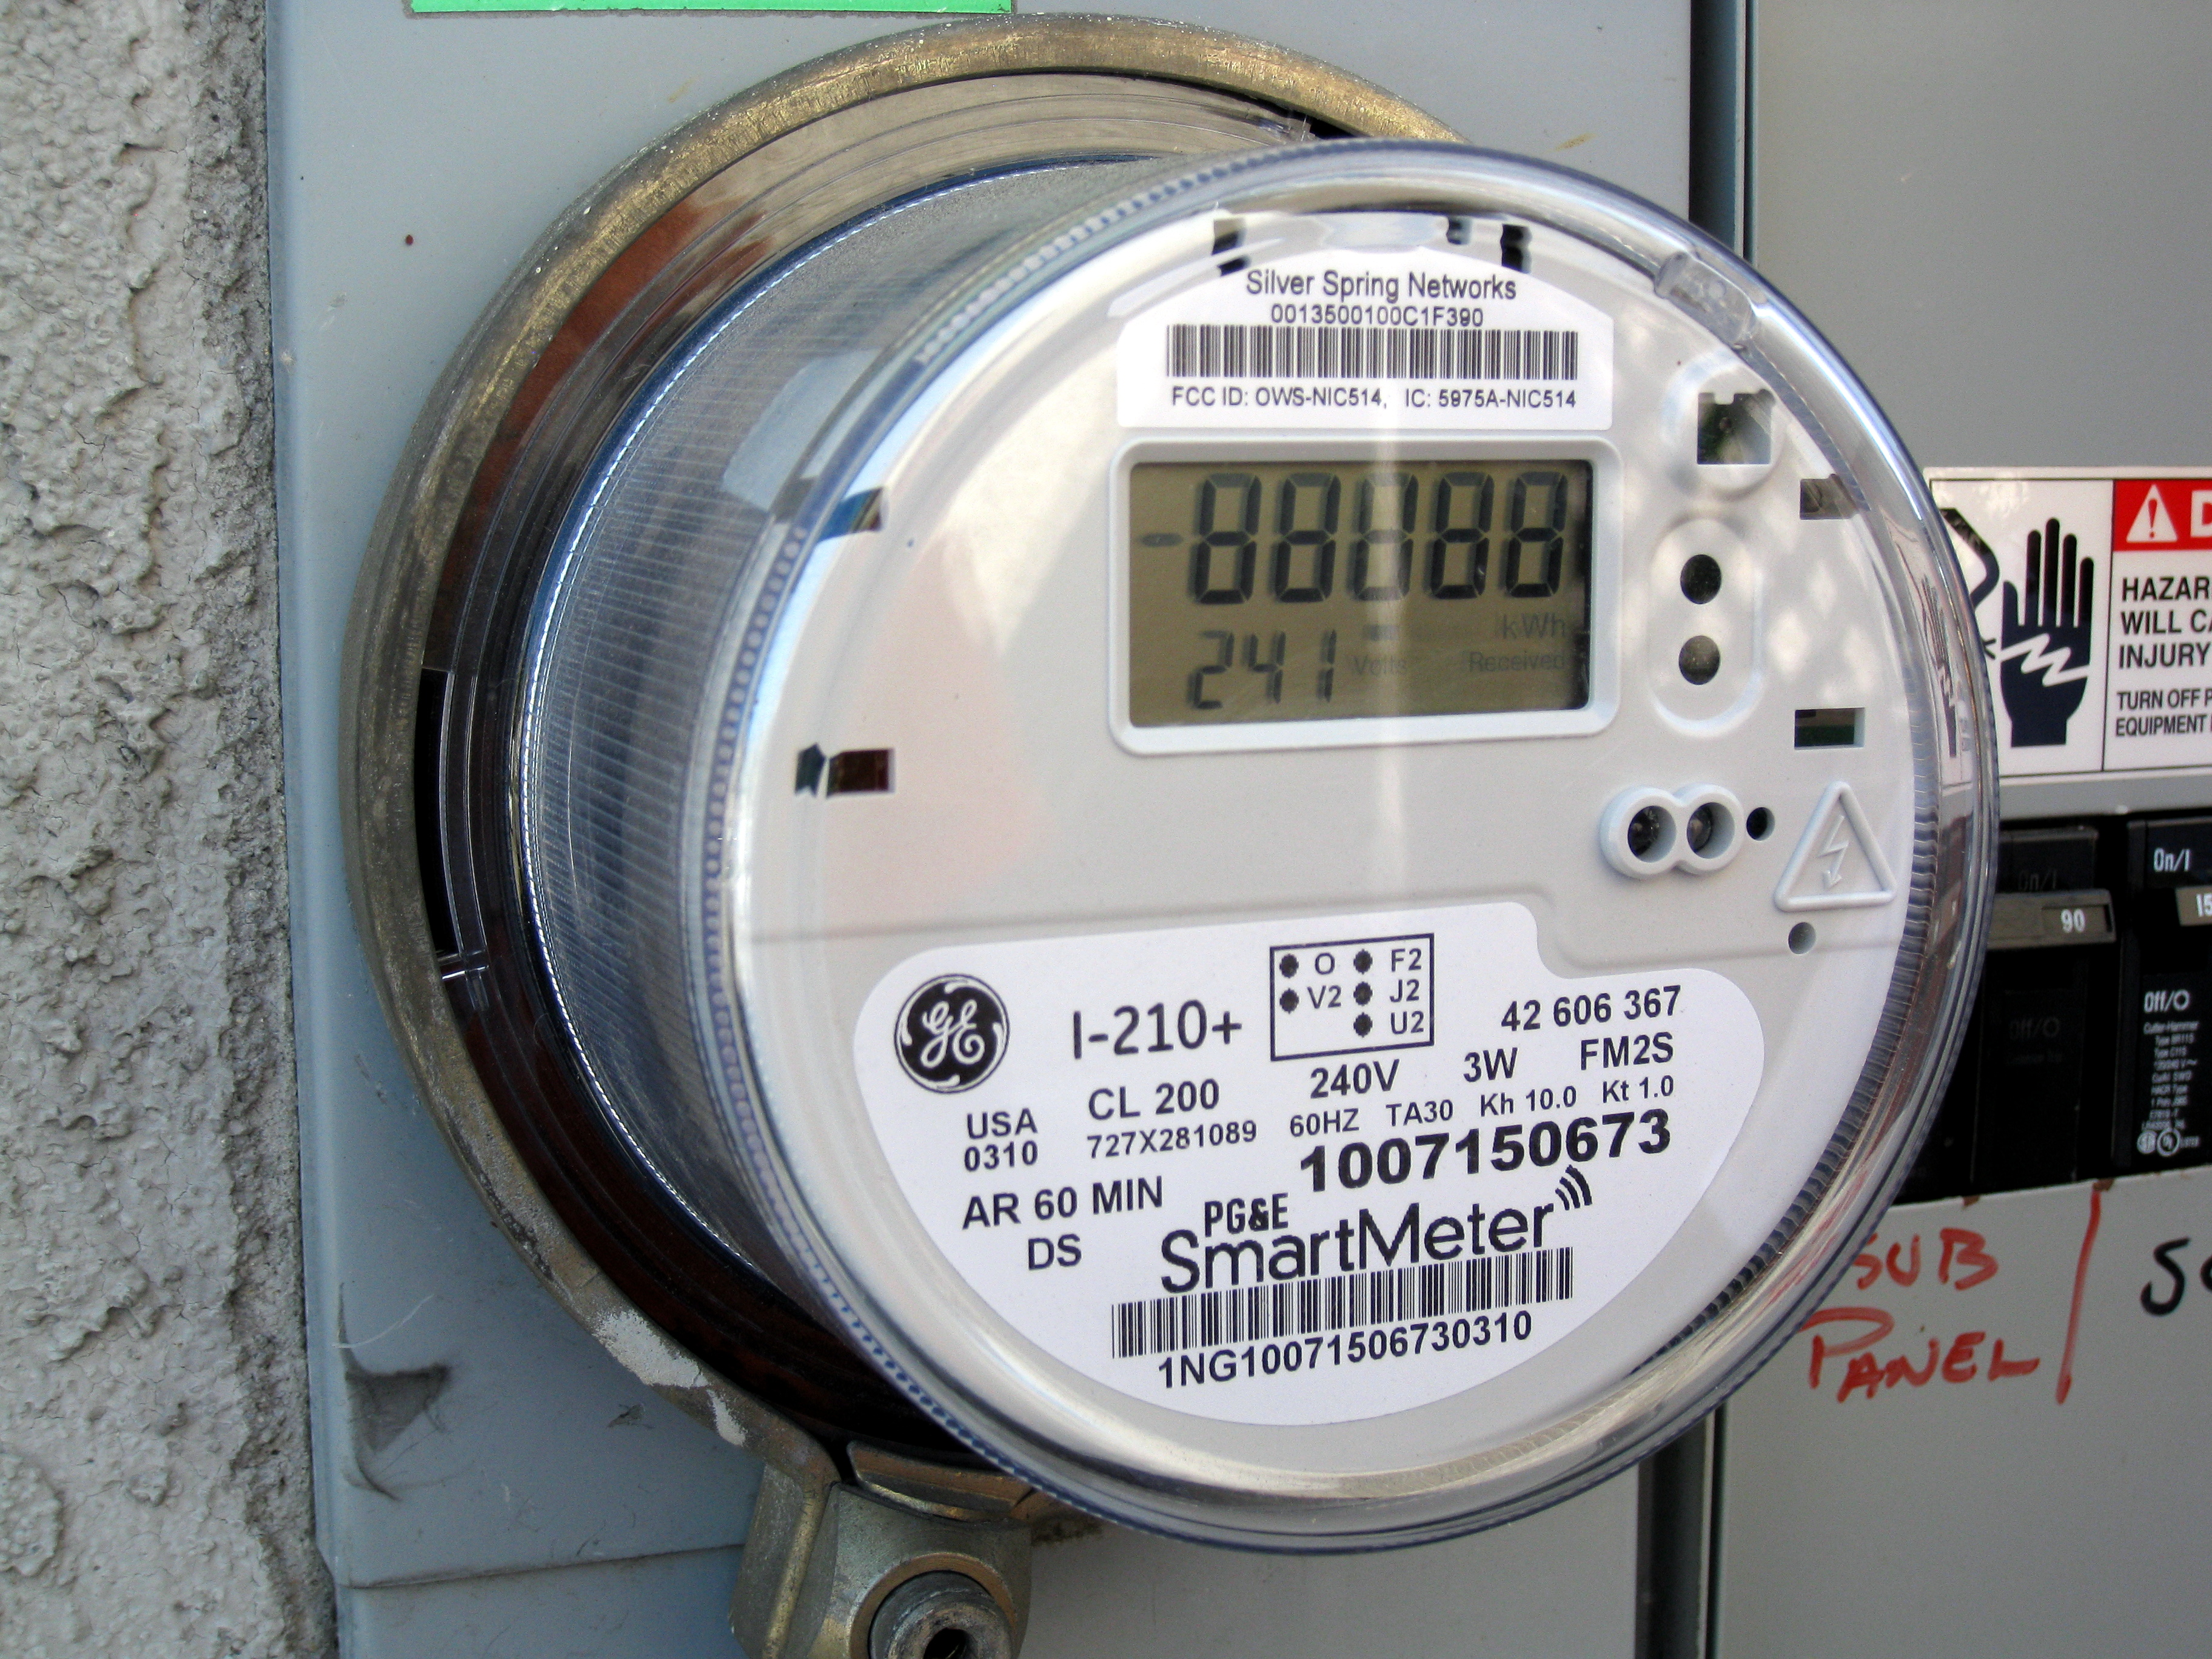
\includegraphics[width=.5\textwidth]{graphics/smart_meter.jpg}

\begin{minipage}{6in}
  
  $\vcenter{\hbox{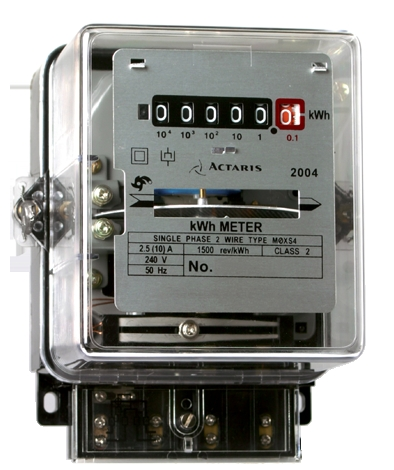
\includegraphics[height=2.25in]{graphics/electrical_meter.jpg}}}$
  \hspace*{.2in}
  $\vcenter{\hbox{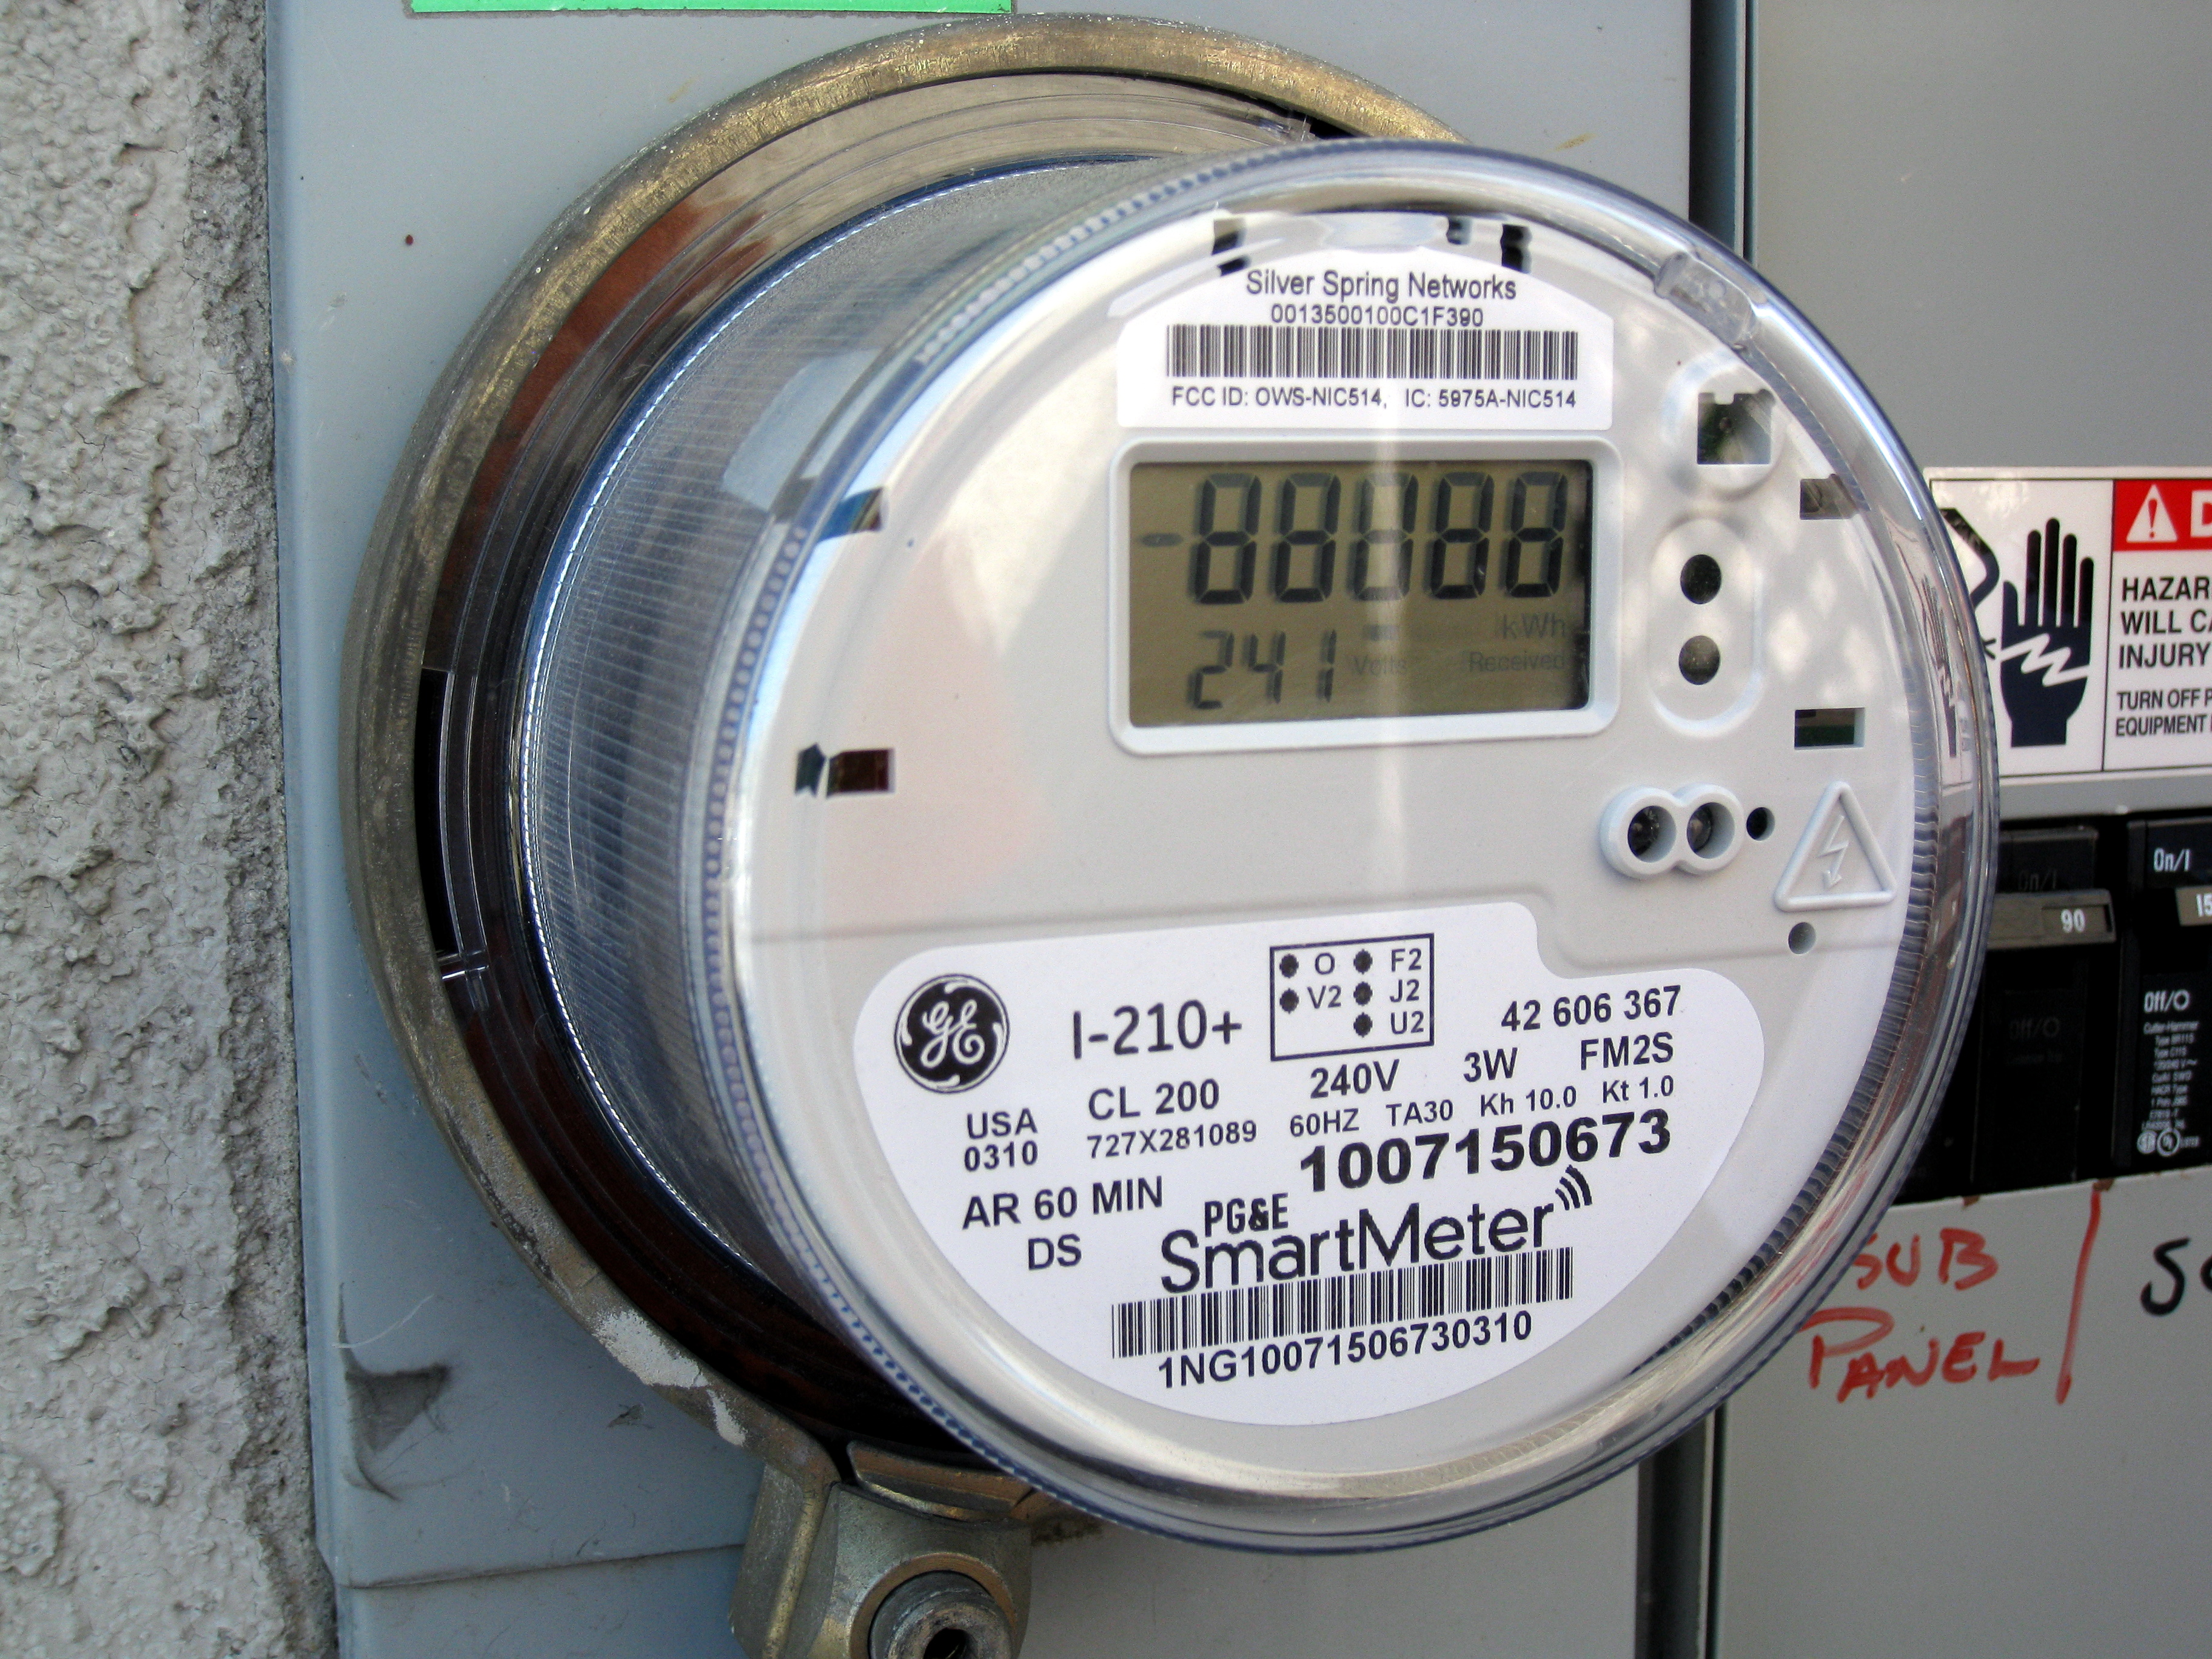
\includegraphics[height=1in]{graphics/smart_meter.jpg}}}$
  
\end{minipage}

\end{frame}

\begin{frame}
  \frametitle{Smart Grid Overview}
  \begin{center}
    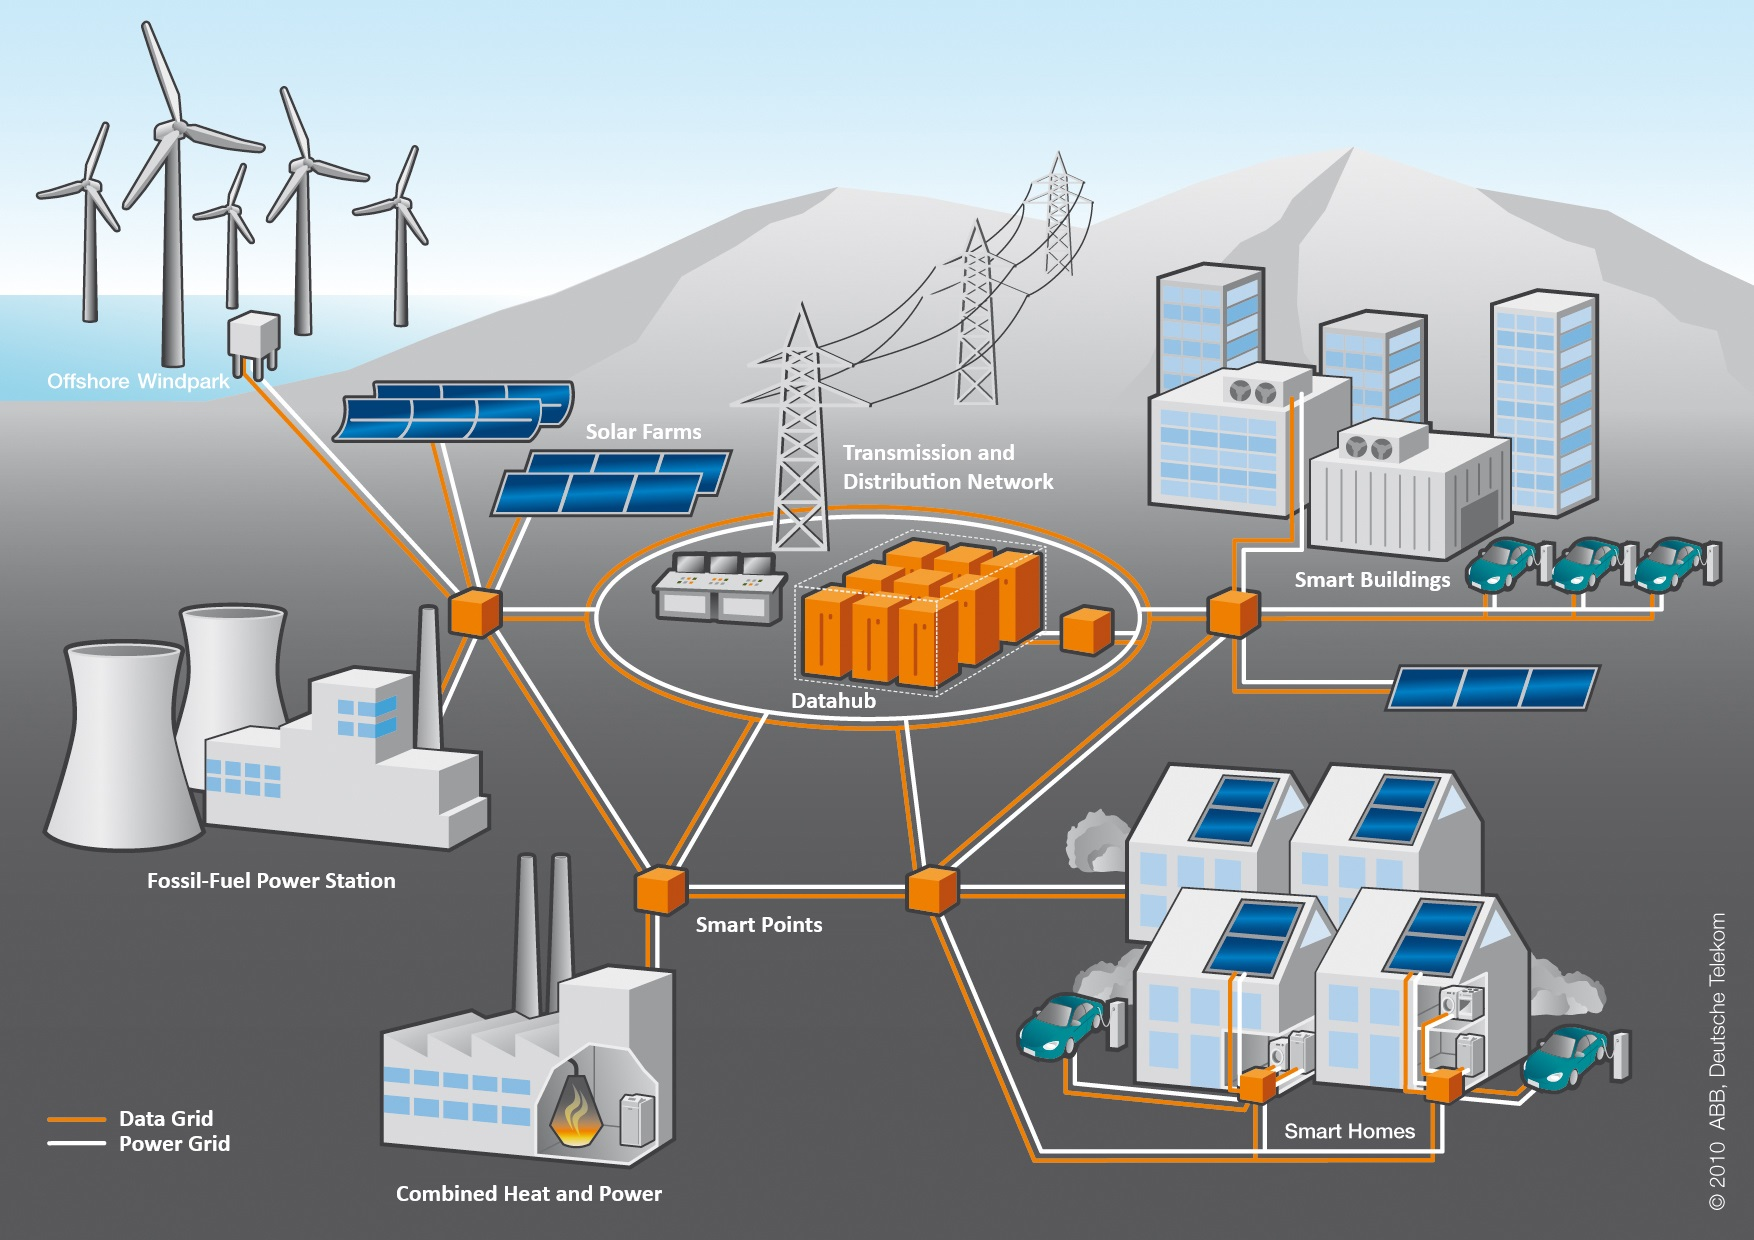
\includegraphics[width=.9\textwidth]{graphics/smart_grid_overview.jpg}
  \end{center}
\end{frame}

\begin{frame}
  \frametitle{Different Architectures}
  \begin{itemize}
	\item \textbf{Italy} -- Regulated monopoly (supplier and distributor is the same).
	\item \textbf{Germany} -- Free market for both distributor and supplier, households will have free choice in both.
	\item \textbf{UK} -- Centralized government-licensed monopoly, which will have a data hub from which data will be distributed to suppliers, customers, etc.
	\item \textbf{Denmark} -- Centralized through 60 government-regulated distributors, a government-owned data hub contains all data.
\end{itemize}

\end{frame}

\begin{frame}
  \frametitle{Smart Meter System}
  \includegraphics{graphics/system.tikz}
\end{frame}

\begin{frame}
  \frametitle{Privacy Concerns}
  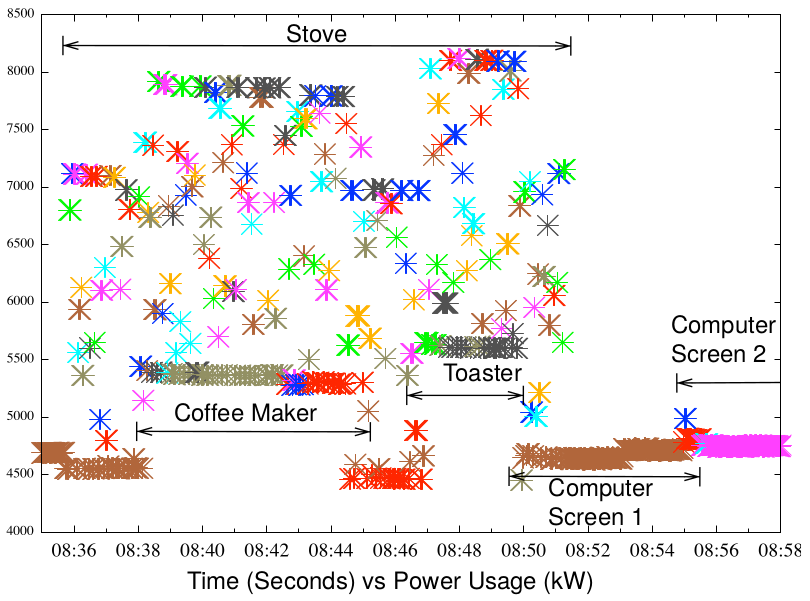
\includegraphics[width=.8\textwidth]{graphics/detailed.png}
\end{frame}

\begin{frame}
  \frametitle{Remote Access-ability}
  \begin{itemize}
  \item Remote switch
  \item Possible attackers:
    \begin{itemize}
    \item States
    \item Terrorists
    \item Environmental activists
    \item Criminals
    \end{itemize}
  \end{itemize}
\end{frame}

\begin{frame}
  \frametitle{Smart Meter Context Model}
  \includegraphics{graphics/smart_meter_context_model.tikz}
\end{frame}
